
\documentclass{IEEEtran}

\usepackage{cite}

\setlength{\parskip}{0.35em}

\usepackage{titlesec} 
\usepackage{url}
\titlespacing{\section}{0pt}{10pt}{6pt} \titlespacing{\subsection}{0pt}{8pt}{4pt}

\usepackage{balance}
\usepackage{float}
\usepackage{graphicx}
\usepackage{amsmath}
\usepackage{xcolor}
\usepackage{enumitem}
\usepackage[colorlinks=true, urlcolor=blue, linkcolor=black, citecolor=black]{hyperref}
\usepackage[colorlinks=true, linkcolor=blue, citecolor=blue, urlcolor=blue]{hyperref}

\usepackage{fancyhdr}

\fancypagestyle{plain}{
    \fancyhf{}
    \fancyfoot[R]{\thepage}
    \renewcommand{\headrulewidth}{0pt}
    \renewcommand{\footrulewidth}{0pt}
}

\pagestyle{plain}


\begin{document}
\raggedbottom

\title{AI-Assisted Reading Support vs Highlighting}

\author{
\IEEEauthorblockN{Roman Andrei, Bianca-Maria Andreica}

\IEEEauthorblockA{Department of Computer Science\\
University of Salerno\\
Italy}
}

\maketitle

\begin{abstract}
This paper conducts a comparison of three modes of
reading support for scientific/technical papers: Manual Highlighting, AI Highlighting and Main Ideas Support, and AI Chatbot
Support. A within-subject study has been carried out using 18 subjects who have done the reading tasks, comprehension quizzes, and
feedback surveys in all three modes. There is no statistically significant difference in quiz score, SUS usability score, and weighted
workload according to the reading support mode. However, AI
Highlighting and Main Ideas Support achieved the shortest reading time and total task time, whereas AI Chatbot Support got the
highest descriptive quiz score. These results suggest that reading assistance through AI does not add to the user’s perceived workload and, at the same time, does not affect comprehension in any mode. Although the differences in comprehension were insignificant.
Index Terms—AI-assisted reading, highlighting, chatbot support, reading comprehension, usability, workload.
\end{abstract}

\begin{IEEEkeywords}
AI-assisted reading, highlighting, chatbot support, reading comprehension, usability, workload.
\end{IEEEkeywords}

\thispagestyle{plain}
\pagestyle{plain}


\section{Introduction}

Scientific and technical articles are packed with complex information, terminology and concepts that are challenging for readers to understand. Reading support solutions including highlighting, annotations, and AI-based assistance can help readers to spot significant information and engage more actively in interaction with the text.

Traditionally, highlighting lets readers pick relevant information, but this method relies on reader’s ability to recognize key ideas in the text. Modern AI-based tools include automatic highlighting of information, explanation of main ideas, summarization, glossary of terms or even question answering through chatbot interaction. At the same time, it is still essential to investigate whether these additional AI-based support methods really make any difference by improving reading comprehension, decreasing task completion time or influencing perceived usability and workload of a reader.

The current research investigates three different modes of reading support, which include Manual Highlighting, AI Highlighting & Main Ideas Support, and AI Chatbot Interaction. The within-subject experiment was conducted with 18 participants completing reading tasks, comprehension quiz and filling in feedback questionnaire in all modes. This experiment will measure quiz performance, task completion time, interaction behavior, usability and perceived workload of participants.

The paper is organized in the following way. Related Work in the field of highlighting and annotation tools as well as AI-assisted reading is discussed in section II. Experiment methodology, participants, materials, experimental conditions, procedure, variables and counterbalancing are described in section III. Results are presented in section IV. Section V is dedicated to discussion and limitation of the research. Possible future work will be outlined in section VI.


\section{Related Work}

There have been many changes made over the years to the various types of digital reading support technologies, which have evolved in three main ways: through visual highlighting, annotations, and new forms of AI-supported reading.

Research in the area of traditional highlighting considered the possibility of improvement in learning outcomes via highlighting as a means of visual stimulation. A meta-analysis of experimental research conducted by Ponce et al.~\cite{ponce2022}, concluded that highlighting might lead to better recall results if the highlighted sections were chosen by instructors rather than by learners. Such fact indicates that it is difficult for learners to identify the most significant pieces of information independently. In turn, Mason et al.~\cite{mason2024} and List and Lin ~\cite{list2023} found out that the efficiency of highlighting highly relies on the selected information, not the act of highlighting itself. Although highlighting can be used as an indicator of learners' engagement and background knowledg e ~\cite{winchell2020}, several studies proved that static highlighting cannot contribute to deeper comprehension and processing of the information.

The process of annotation and the use of social annotation tools is different from basic highlighting since it provides users with additional possibilities for interacting with the text. Interaction may occur through leaving notes and comments, resulting in reflection and production of new knowledge. In social annotation tools, several users can interact with each other by exchanging their annotations. Many researches in the field ~\cite{novak2012, yeh2017, chen2014, johnson2010} show that such approaches may improve learners’ metacognitive skills and thinking. Yeh et al.~\cite{yeh2017}conducted a number of classroom experiments that proved that online annotation helps to improve reading process and its outcomes. Chen and Chen ~\cite{chen2014} also claimed that collaborative annotation improves reading performance. Moreover, Johnson et al.~\cite{johnson2010}  paid attention to the advantages of group-based annotation in higher-order thinking development. Recent work by Omarchevska et al.~\cite{omarchevska2026} proved that these systems require the high levels of cognitive engagement because deeper metacognitive interaction contributes to better learning outcomes.

Recently, researchers became interested in AI-assisted reading support. Such technology allows providing an individual with adaptive assistance based on large language models and intelligent tutoring techniques. AI-based systems include Chat-PRCS ~\cite{wang2024} and intelligent tutoring frameworks ~\cite{xu2019, wijekumar2013} Unlike previous forms of assistance, such systems allow for more dynamic interactions with an individual. Lin et al.~\cite{lin2025} evaluated an AI-supported pre-reading scaffolding system in controlled experiments and found out that this approach improved learners' reading comprehension and motivation. Meanwhile, Feng ~\cite{feng2025}  found out that although AI-assisted strategies lead to the improvement of learning outcomes, inappropriate design of such systems might increase cognitive load. Such systems as Scim ~\cite{fok2023}and IRead ~\cite{zhang2025} aim at increasing reading efficiency through intelligent skimming and combined visual-textual support.

However, a significant limitation of the existing research exists. Most of the studies consider one type of digital assistance (highlighting, annotation, social annotation systems, or AI-assisted reading tool) and evaluate their performance separately, using different experimental designs. Literature review indicates that static highlighting ~\cite{ponce2022, mason2024, list2023} does not provide enough adaptation capabilities to adapt to individual readers, while annotation systems ~\cite{novak2012, chen2014} require active participation from users. At the same time, AI-based methods ~\cite{lin2025, wang2024, zhang2025}, are aimed at providing learners with more flexibility and interactivity.

In addition, comparative analysis of these methods is rather limited and there are few studies that evaluate the efficiency of these tools in controlled conditions. In most of the existing studies, reading comprehension is evaluated through performance-based methods (comprehension questions, recall tests, etc.), which make it possible to conduct a comparative analysis of findings obtained via various research methods. In this context, the current study evaluates richer AI-assisted reading interface compared to traditional highlighting regarding their effects on reading comprehension.

\section{Methodology}

\subsection{Study Design}

In this experiment, within-subject design was used,
which involved two key within-subject factors. First, there was
the mode of reading support that involved three levels, namely
Manual Highlighting, AI Highlighting and Main Ideas Support,
and AI Chatbot Support. Second, there was the article involving
three levels based on the use of three scientific and technical
articles in this experiment. Independent variables were the reading
support mode and the article, while dependent variables included
quiz score, reading time, total task time, interaction metrics,
usability score, and perceived workload. Among others, the interaction
metrics comprised manual highlights, removed highlights, AI
highlights, and chatbot questions.
It is reasonable to use the within-subject design in this
study since participants might differ in their reading speed, prior
knowledge, English language proficiency, familiarity with scientific
and technical terms, and their experience with web applications.
Since all participants completed all three reading support condi-
tions, the impact of individual differences was minimized when
comparing the modes.
The procedure of counterbalancing was used in this study
to avoid order effects that can appear due to the possible increase
in the participants' proficiency in performing the task or fatigue
when doing the task. Order effects are presented in Table I.

\subsection{Research Questions}

The study seeks to address the following research questions:

\begin{itemize}
    \item \textbf{RQ1:} How does the type of reading support influence participants' comprehension of scientific and technical articles?
    \item \textbf{RQ2:} How do Manual Highlighting, AI Highlighting and Main Ideas Support, and AI Chatbot Support differ in terms of task completion time?
    \item \textbf{RQ3:} How do participants interact with each reading support mode in terms of manual highlights, AI highlights, and chatbot questions?
    \item \textbf{RQ4:} How do participants perceive the usability, usefulness and workload of the three reading support modes?
    \item \textbf{RQ5:} Does the article being read influence comprehension scores, task completion time, or interaction behaviour?

\end{itemize}


\subsection{Participants}

In the final sample, there were 18 participants. Participants were college or university students who could comprehend scientific and technology-related articles in English. They had basic experience using a web browser. Any previous experience with browser extensions and digital highlighting systems was not required.

The average age of participants was 21.94 years (SD = 2.10). Ages ranged from 19 to 27 years. There were 8 females (44.4\%) and 10 males (55.6\%) among participants.

The majority of participants studied for Bachelor's degree (61.1\%), then Master's degree (33.3\%) and PhD (5.6\%). Participants studied in different fields, such as computer science, engineering, economics, sociology, law, and other areas.

Concerning the English proficiency of participants, the majority of them had an intermediate or advanced level. In more details, 44.4\% of participants had a B2 level, 33.3\% - C1 level, and 11.1\% had C2 level. In addition, 5.6\% of participants had A1 level, and 5.6\% had B1 level.

Participants were aware about the AI tools. On the scale of 1 to 5, where 1 means 'do not know', and 5 - 'very familiar', 55.6\% of participants chose the highest level, 38.9\% - level 4, and 5.6\% - level 3. Moreover, 83.3\% of participants reported they used chatbots to understand learning material. Nevertheless, most of the participants had no experience with digital highlighting or annotation tools, 66.7\% answered 'no', 16.7\% - 'yes', and 16.7\% - 'not sure'.

Each participant had an anonymous Participant ID. It was used to connect participants' answers to demographic questionnaires, results of tasks, interaction metrics and feedback without recording participants' names. It was also used by the system to assign the counterbalanced article and condition sequence, see Table~\ref{tab:counterbalancing}.

Firstly, participants filled out an initial demographic questionnaire. It contained basic information about participants, such as age, gender, field of study, current level of study, self-evaluated English proficiency, familiarity with AI tools, reading experience with scientific or technical articles and highlighting, annotation tools or chatbots for learning.

\subsection{Materials}

Three English-language scientific or technology-based articles are used in this study.

All three articles are used in every reading task for all participants and the order of articles is counterbalanced across the participants.

The articles used in this study are:

\begin{enumerate}

\item \textbf{``Webb's Scientific Instruments''}. 
Published by NASA Science, this article deals with topics such as space telescopes, observation instruments, and science instrument data collection. The article talks about the scientific instruments of the James Webb Space Telescope and their function in the process of light collection and analysis. Available at the \href{https://science.nasa.gov/mission/webb/science-overview/science-explainers/webbs-scientific-instruments/}{NASA Science website}.

\item \textbf{``A `Robot Pizza Chef' Serving Up Better Quantum Computers''}. 
Published by Berkeley Lab, this article covers the topics of quantum computers, robotic fabrication, qubits, and AI assistance in material research. The article introduces the reader to robotic fabrication and analysis systems that serve as the basis for research into components of quantum computing, such as qubits and Josephson junctions. Available at the \href{https://newscenter.lbl.gov/2026/02/11/a-robot-pizza-chef-serving-up-better-quantum-computers/}{Berkeley Lab website}.

\item \textbf{``Fiber computer allows apparel to run apps and `understand' the wearer''}. 
Published by MIT News, this article discusses topics related to smart clothing, wearable computers, sensors, machine learning, and health tracking. The article features a novel fiber-based computer designed to be incorporated into clothing and track a person's physical activities and health-related information. Available on the \href{https://news.mit.edu/2025/fiber-computer-allows-apparel-to-run-apps-and-understand-wearer-0226}{MIT News website}.

\end{enumerate}

Each article has a predefined multiple-choice quiz. These quizzes are not generated dynamically during the experiment. Therefore, all participants complete the same questions for each article, regardless of the reading support mode applied to that article.

\subsection{Comprehension Quizzes}

Each article had a predefined multiple-choice quiz with 10 questions. The quizzes were not generated dynamically during the experiment. Therefore, all participants answered the same questions for each article, regardless of the reading support mode assigned to that article. The questions assessed factual understanding and comprehension of the article content. The full list of quiz questions is provided in \hyperref[app:quiz_questions]{Appendix~\ref*{app:quiz_questions}}.


\subsection{Experimental Conditions}

There are three experimental conditions in this experiment.

\noindent\textbf{1. Manual Highlighting.} In the Manual Highlighting condition, participants read the article and highlight the part of the text that they find important. After selecting the text, participants can choose the color for highlighting from a floating palette. This condition involves making independent decisions regarding what information is important and should be highlighted.

This experimental condition is used as the baseline reading support mode. This condition represents familiar method of active reading in which the participant decides what information needs to be highlighted.


\begin{figure}[H]
\centering
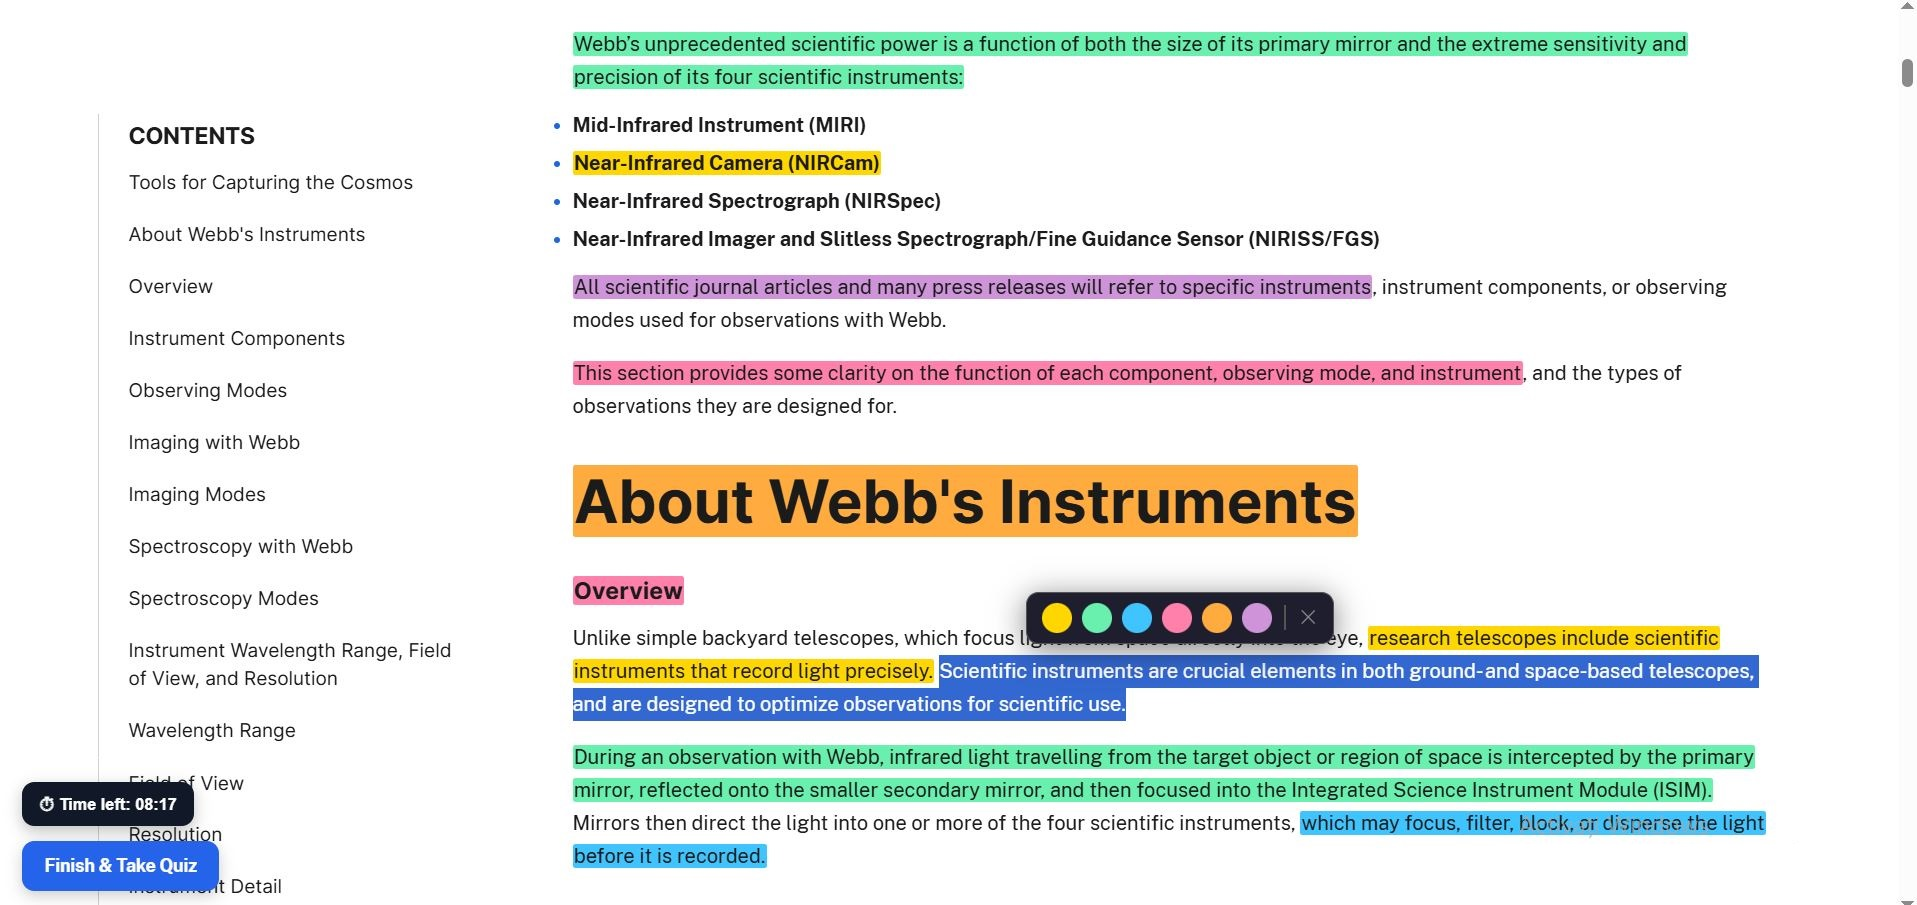
\includegraphics[width=\linewidth]{figures/manual_highlighting.jpg}
\caption{Manual Highlighting mode, where participants select text and choose a highlight colour from the floating palette.}
\label{fig:manual-highlighting}
\end{figure}

\noindent\textbf{2. AI Highlighting and Main Ideas Support.} In the AI Highlighting and Main Ideas Support condition, the system analyzes the article and gives reading support. The interface highlights important parts of the article and shows the panel with focus of the article, main ideas, explanations, key terms, and a takeaway.

This condition provides reading support without requiring the participant to ask questions. The goal of this condition is to investigate if the automatically generated highlights and reading guidance helps participants to comprehend the article.


\begin{figure}[H]
\centering
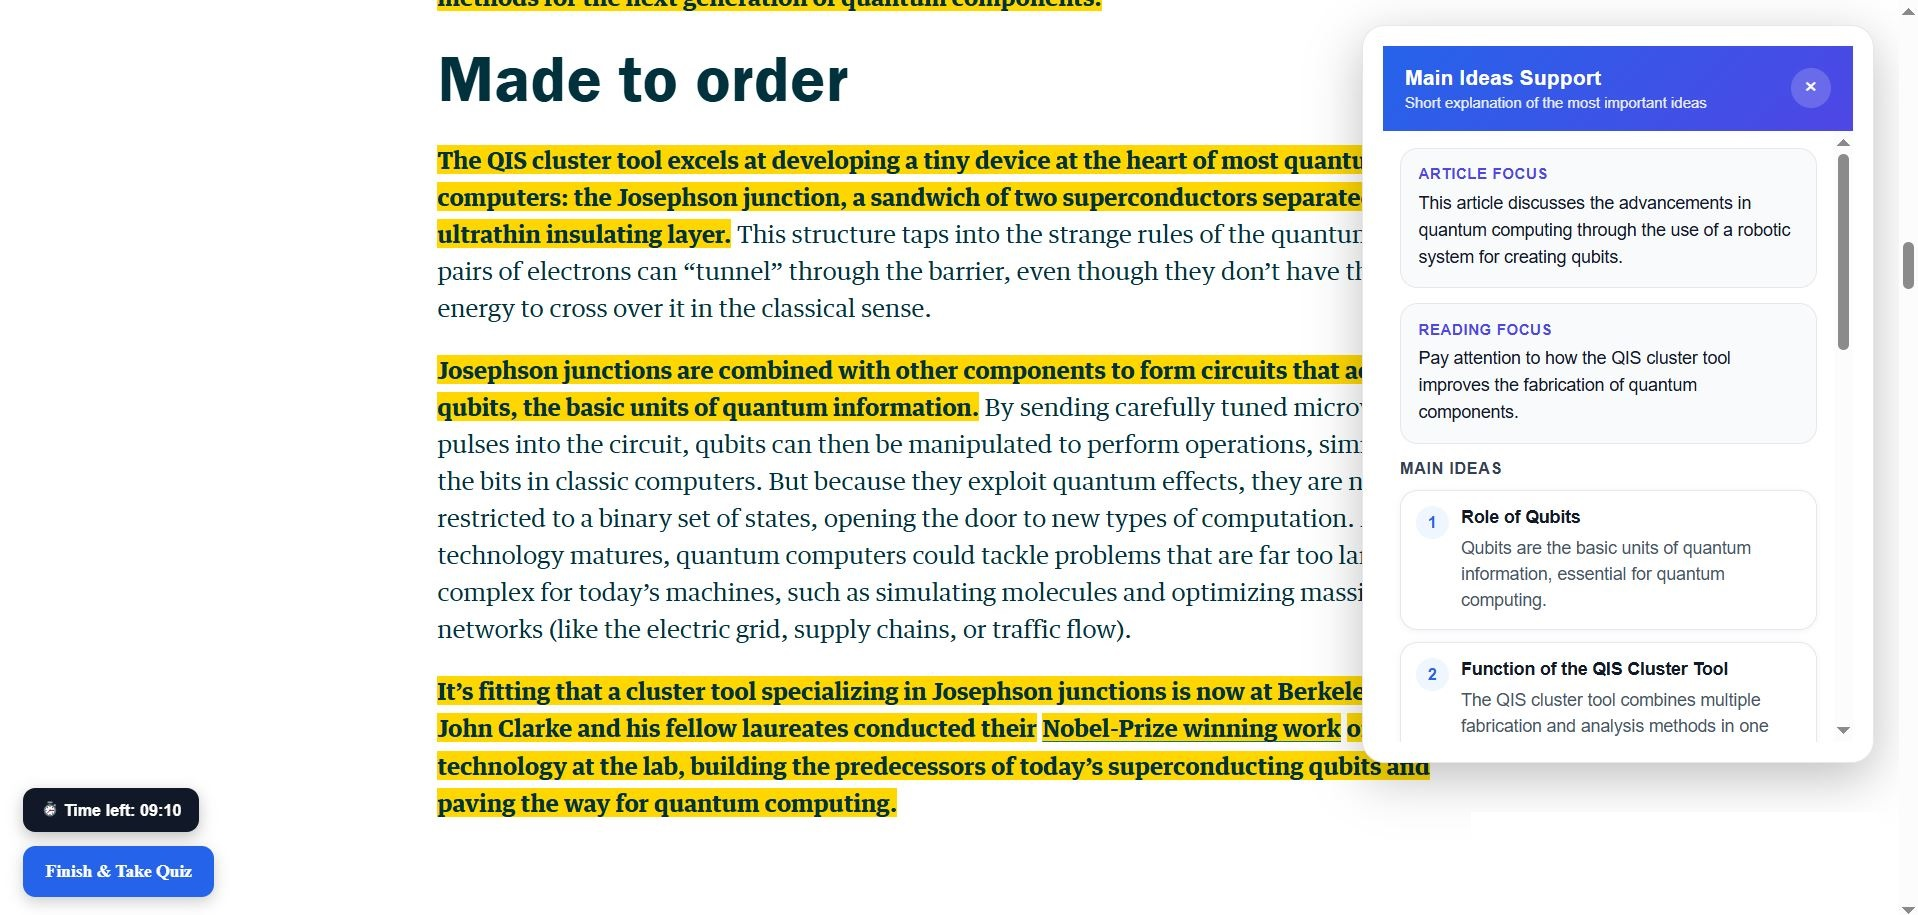
\includegraphics[width=\linewidth]{figures/ai_highlighting_main_ideas.jpg}
\caption{AI Highlighting and Main Ideas Support mode, showing automatic highlights and the side panel with key ideas and takeaways.}
\label{fig:ai-main-ideas}
\end{figure}

\noindent\textbf{3. AI Chatbot Support.} In the AI Chatbot Support condition, participants interact with the chatbot while reading the article. They can ask questions and receive explanations about the article content from the system. The chatbot is able to clarify confusing concepts and technical terms, and help with active inquiry during reading.

Chatbot can help with understanding images and figures present in the article using available captions, alt text, and nearby article text. This experimental condition differs from the previous one by the fact that participants ask their own questions.


\begin{figure}[H]
\centering
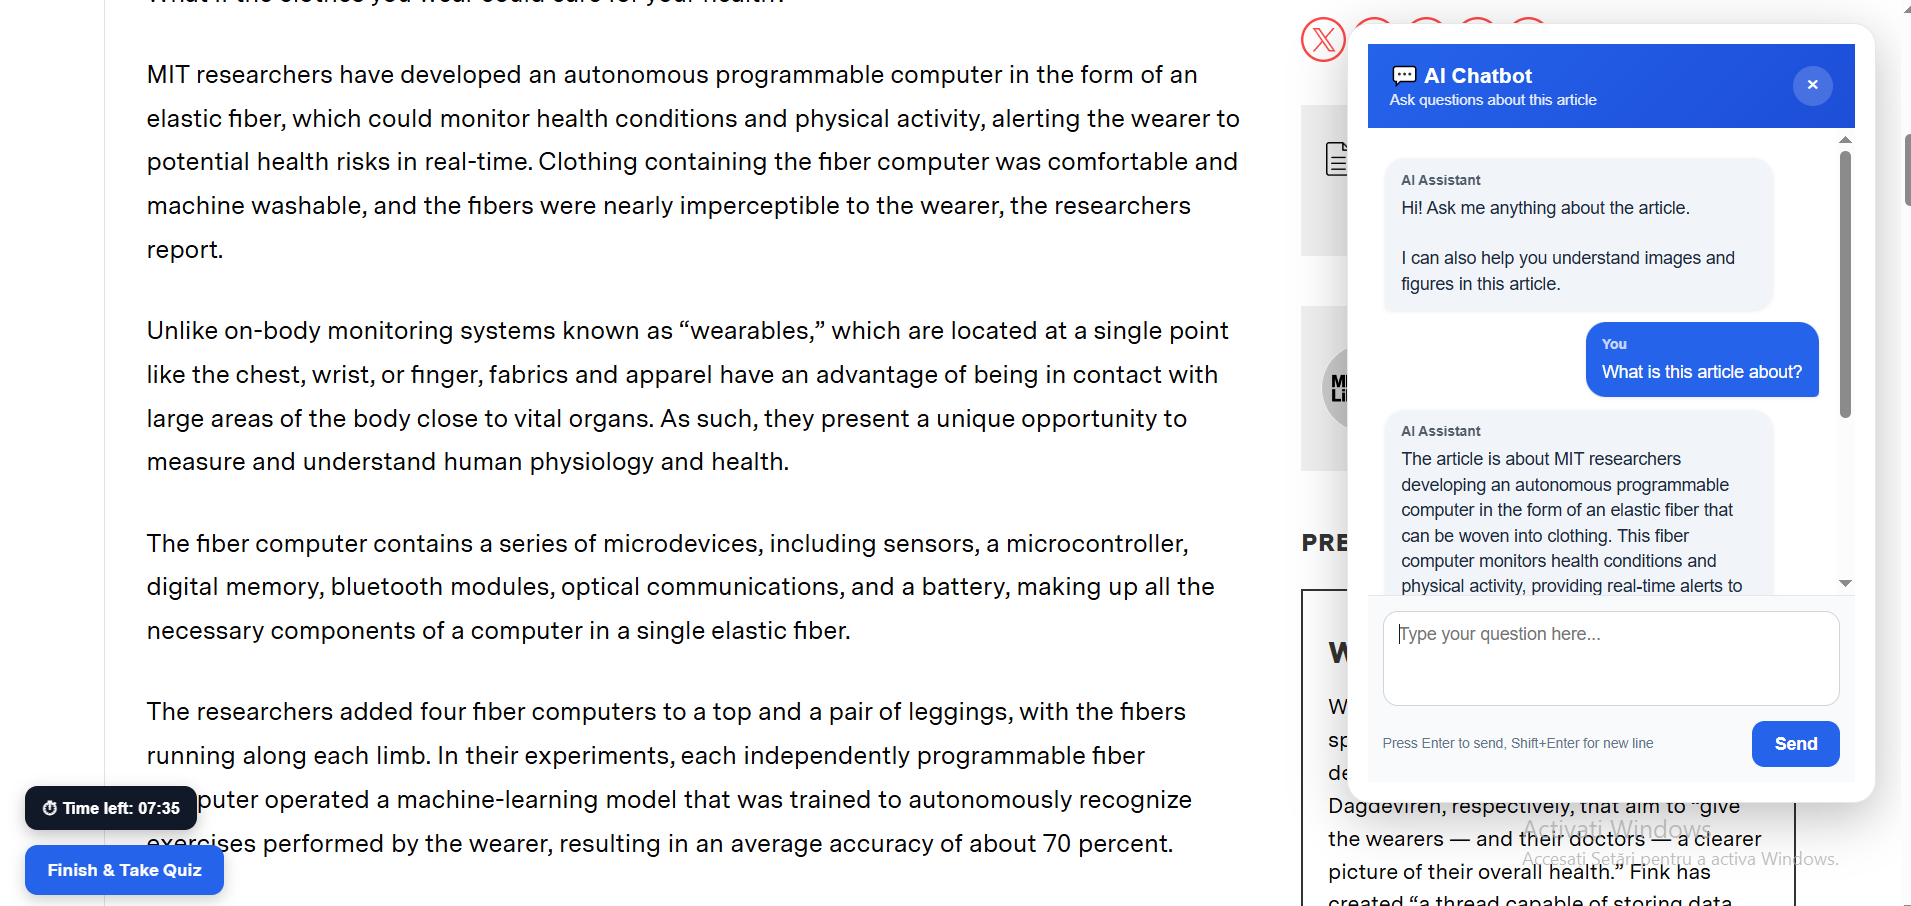
\includegraphics[width=\linewidth]{figures/ai_chatbot_support.jpg}
\caption{AI Chatbot Support mode, where participants ask questions about the article through the chatbot panel.}
\label{fig:ai-chatbot-support}
\end{figure}

\subsection{Procedure}


The experiment was conducted using the laboratory computer. The computing platform on which the experiment took place was a Lenovo ThinkCentre M75q Gen 5 Tiny (AMD). This computer had been set up to have an AMD Ryzen 7 PRO processor, (3.4 GHz, up to 5.0 GHz), 8 GB DDR5-5200 MT/s SODIMM RAM, and integrated graphics. The operating system used during the experiment was and Ubuntu 22.04 LTS. The Flask application was launched locally, and the browser extension was installed in the web browser used in the experiment.

Once the participants landed on the experiment homepage, they put in their Participant ID. Based on the Participant ID supplied by the participants, the system generated a counterbalancing sequence for the reading assistance conditions and articles, as illustrated in Table~\ref{tab:counterbalancing}. The Participant ID used throughout the experiment remained constant.

Before performing any reading tasks, participants fill in the preliminary demographic questionnaire via Google Forms. Access to this questionnaire is available via a link on the experiment home page. Participant ID will be specified in the form in order to link questionnaire responses to anonymous experimental data collected by the application. The first article will remain locked until the questionnaire step is completed.


\begin{figure}[H]
\centering
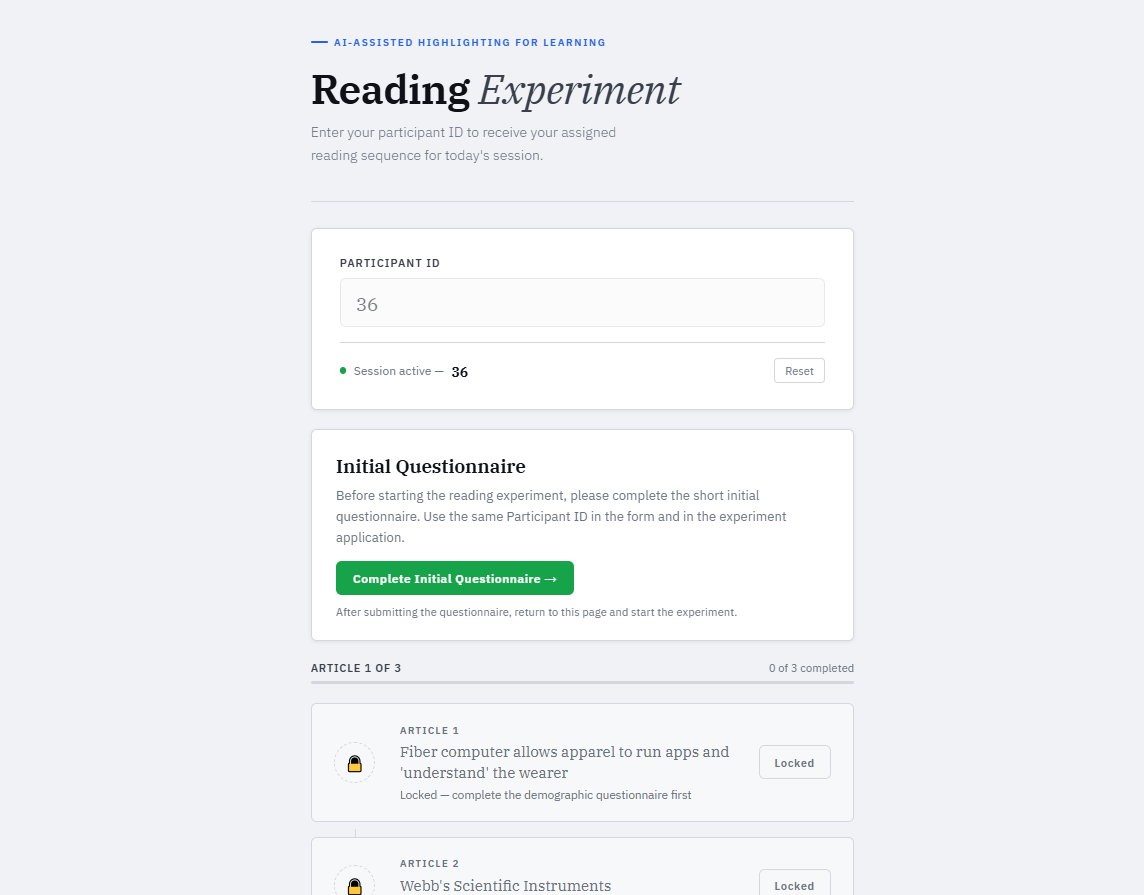
\includegraphics[width=\linewidth]{figures/experiment_homepage.jpg}
\caption{Experiment homepage showing the Participant ID input, article sequence, and task progress.}
\label{fig:experiment-homepage}
\end{figure}

For each task, participants open the article allocated for the task and perform it with the help of the allocated reading support condition (Manual Highlighting, AI Highlighting and Main Ideas Support, or AI Chatbot Support).

After completing the reading task, participants take an integrated comprehension quiz for the article. The quiz is displayed in the form of a modal window above the article page. While answering the questions in the quiz, the reading support options cannot be used, so the participants answer the questions based on their understanding of the article. After completing the quiz, the application saves the quiz result and interaction metrics obtained in the course of the task. Participants can change their choice as long as they do not submit the quiz and at the end the answers will be sent in a JSON file, without allowing the user to review.

After completing the comprehension quiz, participants return to the experiment home page. At this point, the next article will still be locked. In its place, a short feedback form for the current reading mode will become available. This feedback form is integrated into the application and is displayed as a modal window. It includes both SUS-style usability items and NASA-TLX-style workload items, but it is shown to the participants as a short reading mode feedback form.

Only after the per-mode feedback form is submitted, the application unlocks the next article. In such a way, for each reading support mode, the system receives not only comprehension data but also usability and workload feedback.

The same procedure is performed three times. After the completion of the third comprehension quiz and the third per-mode feedback form, the final comparative feedback questionnaire will become available. This questionnaire will be completed via Google Forms and will ask participants to compare three reading support modes.

\subsection{Questionnaires}

This study uses three questionnaire components:

\subsubsection{Initial Demographic Questionnaire}

The initial demographic questionnaire is given before reading tasks. It collects basic participant background that could be used in interpreting study results.

The Participant ID is included in the form in order to match questionnaire responses with the experimental data collected anonymously by the application.

The initial questionnaire contains items such as:

\begin{itemize}
    \item participant ID;
    \item consent to the processing of personal data for the purpose of participating the experiment;
    \item age;
    \item gender or “prefer not to say”;
    \item academic field/study programme;
    \item level of English language skills;
    \item familiarity with scientific/technical literature;
    \item familiarity with artificial intelligence technologies;
    \item previous usage of digital highlighting/annotation tools;
    \item previous usage of chatbots for education.
    
\end{itemize}

\subsubsection{Per-Mode Feedback Questionnaire}

At the end of every comprehension quiz, the participant fills out a brief questionnaire regarding the current reading mode. The questionnaire is embedded into the application interface and is displayed in a popup on the experiment page.

Even though the interface presents it as a short feedback form, the questionnaire incorporates both SUS-style usability items and NASA-TLX-style workload items. The reason behind this is collecting quick feedback after each interaction mode in order for the participant to be able to continue on to the next article.

Per-mode feedback questionnaire contains items regarding:

\begin{itemize}
    \item ease of use;
    \item perceived complexity;
    \item confidence while using the mode;
    \item need for help;
     \item integration of the mode’s functions;
     \item confusion;
    \item support for comprehending the article;
    \item readiness to use the mode again;
    \item mental demand;
    \item temporal demand;
    \item effort;
    \item frustration;
    \item performance;
    \item workload;
    \item optional comments on the reading mode.
\end{itemize}

The Per-Mode Feedback Questionnaire was scored as two summary scales: one using the SUS methodology and the other using the NASA-TLX methodology. The SUS-style usability score was calculated on a 0-100 scale. Positive usability statements (e.g., easy to use, feel confident, integrated nature of the mode's functions, comprehension of the article, willingness to use the mode again), were scored directly while negative usability statements (e.g., complicated to use, needed help, confused by the mode) were reverse-scored. The normalized usability score was therefore determined as:

\begin{equation}
SUS_{style} = \frac{\sum_{i=1}^{n} u_i}{4n} \times 100
\end{equation}

where $u_i$ represents the recoded usability item score and $n$ is the number of usability items. This formula converts the recoded Likert-scale responses into a percentage-like score from 0 to 100, where higher values indicate higher perceived usability.

Workload score was measured using NASA-TLX-like criteria which included the following factors: mental demand, temporal demand, effort, frustration, performance, and workload itself. Due to the fact that the more positive performance was, the lower was the perceived workload, the item about performance had been reverse-scored while computing the total workload score:

\begin{equation}
Workload = \frac{MD + TD + E + F + P_{rev} + W}{6}
\end{equation}

where $MD$ represents mental demand, $TD$ is temporal demand, $E$ is effort, $F$ is frustration, $P_{rev}$ represents performance score coded in the reverse manner, and $W$ stands for overall workload. High values of workload represent high perceptions of workload.

\subsubsection{Final Comparative Feedback Questionnaire}

The last questionnaire can be answered only when all three reading tasks, comprehension quizzes, and per-mode feedback forms have been completed. This questionnaire is also conducted through Google Forms.

In contrast to per-mode feedback questionnaire, the last one does not require evaluation of each of the three modes separately again with detailed usability questions. Instead, participants are required to compare these three modes.

Final comparative questionnaire consists of items like:

\begin{itemize}
    \item which mode provided better understanding of the articles;
    \item which mode was easier to use;
    \item which mode seemed more helpful in terms of studying;
    \item which mode seemed to be more distracting;
     \item which mode participants would prefer to use again;
     \item what participants liked the most about the system;
    \item what participants would change about it;
    \item additional comments regarding the experiment.
    
\end{itemize}

\subsection{Collected Metrics}

The independent variables were reading support mode and article while the dependent variables were quiz score, reading time, total task time, usability score, workload score, and interaction behavior.

The application automatically saved all the data in JSON files, including quiz results and interaction measures. They included quiz score, number of correct answers in the quiz, reading time before opening the quiz, total task time, time limit reached, number of manual highlights made, number of manual highlights removed, number of AI highlights made, and the number of chatbot questions.

Feedback regarding usability and workload of per mode were saved separately whereas chatbot interactions were recorded in a separate chatbot log file. It contained the Participant ID, Article details, participant questions to the chatbot, and chatbot answers.

All the collected data were then exported to an Excel spreadsheet which had data tables, summary tables, and charts for comprehension scores, task duration, interaction behavior, usability feedback, workload feedback, and chatbot interactions.

\subsection{Statistical Analysis}

For the analysis of data, AnovaGUI software package was used. One input file for each dependent variable was created. It consisted of 18 rows corresponding to 18 participants that were involved into the analysis and three columns corresponding to the three levels of the within-subjects factor.

In case of the analyses based on the reading support modes, the within-subjects factor was Mode, consisting of three levels: Manual Highlighting (MH), AI Highlighting and Main Ideas Support (AIM) and AI Chatbot Support (CHAT). Such organization was applied to the following variables: quiz score, reading time, total task time, SUS usability score and weighted NASA workload. In case of the article analysis, the within-subjects factor was Article and also had three levels: Article 1, Article 2 and Article 3.

In AnovaGUI, the number of participants was fixed at 18 and F1 (within-subjects factor) was fixed at 3 levels. Options like ANOVA table, main effect means, effect sizes, summary statements and the option without verbose information were checked. The output results were represented by means of F statistic, degrees of freedom, p-value and partial eta-squared ($\eta_p^2$). Descriptive statistics were calculated in terms of mean and standard deviation.

Input files and output results of ANOVA analysis were added to the project repository in order to make the statistical analysis reproducible.


\subsection{Counterbalancing}

The counterbalanced design that was applied for the final experiment is presented in \hyperref[tab:counterbalancing]{Table~\ref*{tab:counterbalancing}}. The table includes the information about the article sequence and reading condition sequence for each subject. This design was applied in order to minimize the potential order effects connected with familiarity, fatigue, and article complexity.

\begin{table}[H]
\centering
\caption{Counterbalanced article and condition order structure used in the final analysis}
\label{tab:counterbalancing}
\label{tab:counterbalancing}
\scriptsize
\renewcommand{\arraystretch}{1.15}

\begin{tabular}{c c c}
\hline
Participant ID & Article Order & Condition Order \\
\hline
P2  & 1 $\rightarrow$ 2 $\rightarrow$ 3 & MH $\rightarrow$ CHAT $\rightarrow$ AIM \\
P3  & 1 $\rightarrow$ 2 $\rightarrow$ 3 & AIM $\rightarrow$ MH $\rightarrow$ CHAT \\
P4  & 1 $\rightarrow$ 2 $\rightarrow$ 3 & AIM $\rightarrow$ CHAT $\rightarrow$ MH \\
P5  & 1 $\rightarrow$ 2 $\rightarrow$ 3 & CHAT $\rightarrow$ MH $\rightarrow$ AIM \\
P6  & 1 $\rightarrow$ 2 $\rightarrow$ 3 & CHAT $\rightarrow$ AIM $\rightarrow$ MH \\
P7  & 2 $\rightarrow$ 3 $\rightarrow$ 1 & MH $\rightarrow$ AIM $\rightarrow$ CHAT \\
P8  & 2 $\rightarrow$ 3 $\rightarrow$ 1 & MH $\rightarrow$ CHAT $\rightarrow$ AIM \\
P9  & 2 $\rightarrow$ 3 $\rightarrow$ 1 & AIM $\rightarrow$ MH $\rightarrow$ CHAT \\
P10 & 2 $\rightarrow$ 3 $\rightarrow$ 1 & AIM $\rightarrow$ CHAT $\rightarrow$ MH \\
P11 & 2 $\rightarrow$ 3 $\rightarrow$ 1 & CHAT $\rightarrow$ MH $\rightarrow$ AIM \\
P12 & 2 $\rightarrow$ 3 $\rightarrow$ 1 & CHAT $\rightarrow$ AIM $\rightarrow$ MH \\
P13 & 3 $\rightarrow$ 1 $\rightarrow$ 2 & MH $\rightarrow$ AIM $\rightarrow$ CHAT \\
P14 & 3 $\rightarrow$ 1 $\rightarrow$ 2 & MH $\rightarrow$ CHAT $\rightarrow$ AIM \\
P15 & 3 $\rightarrow$ 1 $\rightarrow$ 2 & AIM $\rightarrow$ MH $\rightarrow$ CHAT \\
P16 & 3 $\rightarrow$ 1 $\rightarrow$ 2 & AIM $\rightarrow$ CHAT $\rightarrow$ MH \\
P17 & 3 $\rightarrow$ 1 $\rightarrow$ 2 & CHAT $\rightarrow$ MH $\rightarrow$ AIM \\
P18 & 3 $\rightarrow$ 1 $\rightarrow$ 2 & CHAT $\rightarrow$ AIM $\rightarrow$ MH \\
P19 & 1 $\rightarrow$ 2 $\rightarrow$ 3 & MH $\rightarrow$ AIM $\rightarrow$ CHAT \\
\hline
\end{tabular}

\vspace{1mm}
\begin{minipage}{0.95\columnwidth}
\scriptsize
\raggedright
\textit{Note.} MH = Manual Highlighting; AIM = AI Highlighting and Main Ideas Support; CHAT = AI Chatbot Support.
\end{minipage}

\end{table}


\section{Results}

\subsection{Participants}

The final analysis was done for 18 subjects who
performed all three reading tasks. Therefore, there were a total
of 54 sessions of task performance for the final analysis.
In all three reading support conditions: Manual Highlighting,
AI Highlighting and Main Ideas Support, and AI Chatbot Support,
each subject participated in all three experimental trials.
There was an extra pilot session that was run before the main
experimental trials in order to check the feasibility of the experiment.

\subsection{Comprehension Quiz Performance}

Table~\ref{tab:quiz_by_mode} shows the average quiz scores received in the three reading support modes. Reading support mode AI Chatbot
Support scored the highest average quiz score, which was 88.33
out of 100 points. The average score of reading support mode
Manual Highlighting was 83.89, while reading support mode
AI Highlighting and Main Ideas Support scored 82.78.

A repeated-measures ANOVA was directed to compare quiz scores across the three reading support modes. The effect of reading support mode on quiz
score was not statistically significant, $F(2,34)=0.89$, $p=.421$, $\eta_p^2=.050$. Consequently, although the highest descriptive average score was obtained in the AI Chatbot Support reading support mode, the results do not present statistically significant evidence that one reading support mode resulted in better comprehension than the other two modes.

\begin{table}[H]
\centering
\caption{Average quiz score by reading support mode.}
\label{tab:quiz_by_mode}
\scriptsize
\begin{tabular}{lccc}
\hline
Mode & N & Mean & SD \\
\hline
MH & 18 & 83.89 & 15.39 \\
AIM & 18 & 82.78 & 14.06 \\
CHAT & 18 & 88.33 & 13.39 \\
\hline
\end{tabular}

\vspace{1mm}
\begin{minipage}{0.95\columnwidth}
\scriptsize
\textit{Note.} MH = Manual Highlighting; AIM = AI Highlighting and Main Ideas Support; CHAT = AI Chatbot Support.
\end{minipage}
\end{table}

\subsection{Task Time}

\hyperref[tab:time_by_mode]{Table~\ref*{tab:time_by_mode}} reports the mean and standard deviation for reading time and total task time in the three reading support modes. AI Highlighting and Main Ideas Support required the least amount of reading and total task time on average. Reading support modes Manual Highlighting and AI Chatbot Support require more time on average.

Statistically significant effect of reading support mode
on reading time was found using repeated-measures ANOVA, $F(2,34)=5.33$, $p=.010$, $\eta_p^2=.239$. The effect on total
task time was also found significant, $F(2,34)=3.51$, $p=.041$, $\eta_p^2=.171$.

However, the time data should be interpreted with
caution. In the process of experimentation, some partici-
pants understood the available time as maximum time they
could spend on the task, and not as time pressure condi-
tion. Hence, reaching time limit or spending more time on
the task does not mean that the mode was difficult or less
efficient.

\begin{table}[H]
\centering
\caption{Reading time and total task time by mode.}
\label{tab:time_by_mode}
\scriptsize
\begin{tabular}{lcccc}
\hline
Mode & Reading Mean (s) & Reading SD & Total Mean (s) & Total SD \\
\hline
MH & 519.50 & 182.08 & 704.78 & 196.25 \\
AIM & 397.78 & 166.94 & 581.56 & 194.69 \\
CHAT & 508.06 & 199.56 & 669.78 & 213.61 \\
\hline
\end{tabular}
\end{table}

\subsection{Article Effect}

The results were also analyzed by article. Article 3 obtained the highest average quiz score, followed by Article 2 and Article 1. A repeated-measures ANOVA showed a statistically significant effect of article on quiz score, $F(2,34)=10.63$, $p<.001$, $\eta_p^2=.385$.

This result shows that quiz performance varied across the three articles. Article 3 obtained the highest average score, while Article 1 obtained the lowest average score. This finding also supports the use of counterbalancing in the experimental design, since article order was varied across participants to reduce the influence of article-specific effects on the comparison between reading support modes.

\begin{table}[H]
\centering
\caption{Average quiz score by article.}
\label{tab:quiz_by_article}
\scriptsize
\begin{tabular}{lccc}
\hline
Article & N & Mean & SD \\
\hline
Article 1 & 18 & 77.78 & 14.37 \\
Article 2 & 18 & 83.33 & 14.95 \\
Article 3 & 18 & 93.89 & 7.78 \\
\hline
\end{tabular}
\end{table}

\subsection{Interaction Behaviour}

The application also measured interaction metrics in each condition. Participants made an average of 15.72 highlights in the Manual Highlighting condition. The AI Highlighting and
Main Ideas Support condition generated an average of 26.67 AI Highlights. Participants posed an average of 3.28 chatbot questions in the AI Chatbot Support condition.

Thus, it is clear that these three conditions involved different types of interactions. Manual Highlighting required participants to select information actively, AI Highlighting automatically highlighted relevant information visually, and AI Chatbot Support allowed asking questions.


\begin{table}[H]
\centering
\caption{INTERACTION METRICS BY READING SUPPORT MODE}
\label{tab:interaction_metrics}
\scriptsize
\begin{tabular}{lc}
\hline
Metric & Mean \\
\hline
Manual highlights created in MH & 15.72 \\
AI highlights shown in AIM & 26.67 \\
Chatbot questions asked in CHAT & 3.28 \\
\hline
\end{tabular}
\end{table}

\subsection{Usability and Workload Feedback}

The feedback questionnaire for each mode included SUS-like usability measures and NASA-TLX-like workload measurements. Table~\ref{tab:usability_workload} shows the results for usability and workload averages for each mode. All three modes had high average SUS scores that were very similar to each other.AI Chatbot Support obtained the highest average SUS score 81.39, followed by AI Highlighting and Main Ideas Support – 81.25, and Manual Highlighting – 80.83. There were no statistically significant differences between these modes with regard to SUS score,
 $F(2,34)=0.02$, $p=.983$, $\eta_p^2=.001$.

Average weighted workload scores were also similar in these modes. Manual Highlighting had the highest average workload score of 10.63, followed by AI Highlighting and Main Ideas Support of 9.88, and AI Chatbot Support of 9.65. A repeated measures ANOVA showed no statistically significant differences between modes for weighted workload, $F(2,34)=0.72$, $p=.495$, $\eta_p^2=.041$.

These results imply that all modes were generally usable and that the workload differences between modes were small.

\begin{table}[H]
\centering
\caption{Usability and workload feedback by mode.}
\label{tab:usability_workload}
\scriptsize
\begin{tabular}{lcc}
\hline
Mode & SUS score & Weighted workload \\
\hline
MH & 80.83 & 10.63 \\
AIM & 81.25 & 9.88 \\
CHAT & 81.39 & 9.65 \\
\hline
\end{tabular}
\end{table}

\subsection{Final Comparative Feedback}

Feedback received during the final comparison revealed that the majority of participants perceived the AI-based modes more favorably than Manual Highlighting. Specifically, concerning the question of which mode made it easier for participants to understand the articles, AI Highlighting and Main Ideas Support and AI Chatbot Support were selected by the same number of people, namely, 8 participants (44.4\%), while Manual Highlighting was chosen by only 2 participants (11.1\%).

The participants found the mode AI Highlighting and Main Ideas Support to be the most convenient. Indeed, this option was selected by 13 participants (72.2\%), whereas AI Chatbot Support was selected by 3 participants (16.7\%), and Manual Highlighting – by 2 participants (11.1\%). As for the mode usefulness in terms of studying, AI Chatbot Support was selected by 9 participants (50.0\%), AI Highlighting and Main Ideas Support – by 7 participants (38.9\%), and Manual Highlighting – by 2 participants (11.1\%).

When it comes to the level of distraction associated with these modes, Manual Highlighting and AI Highlighting and Main Ideas Support were selected by the same number of people, namely, 7 participants (38.9\%), while AI Chatbot Support was selected by 4 participants (22.2\%). Finally, as far as preferences for future usage are concerned, 8 participants (44.4\%) chose AI Chatbot Support, 5 participants (27.8\%) chose AI Highlighting and Main Ideas Support, 4 participants (22.2\%) chose Manual Highlighting, and 1 participant (5.6\%) did not want to use any of them.

Therefore, the results of the final comparison suggest that the participants found AI-based modes to be more favorable than Manual Highlighting mode. The most convenient one is AI Highlighting and Main Ideas Support, and the most useful and favored one is AI Chatbot Support.


\subsection{Exploratory Analysis of Demographic Data}

In order to conduct an exploratory analysis of the demographic data, the demographic questionnaire responses and the results of the experiment were connected based on the Participant ID. Average quiz score, average reading time, average total task time, average SUS score, and average weighted NASA workload were calculated for each participant for the three reading tasks.

For numerical variables (age and AI familiarity), Pearson correlations were used; and for ordinal self-report variables (English proficiency and frequency of using AI tools), Spearman correlations were used. Age is not significantly correlated with average quiz score ($r=-0.02$, $p=.953$), average reading time ($r=-0.03$, $p=.907$), or average total task time ($r=-0.01$, $p=.964$).

Similarly, English proficiency is not correlated with average quiz score ($\rho=.17$, $p=.489$) and with the time spent on the task. A weak negative correlation is shown between English proficiency and the weighted workload ($\rho=-.41$, $p=.088$), meaning that participants with higher English proficiency could find the tasks easier.

Familiarity with AI tools is slightly positively correlated with average quiz score ($r=.29$, $p=.247$) and slightly negatively correlated with the weighted workload ($r=-.32$, $p=.193$). Hence, there is a weak association that the more familiar the participants were with AI tools, the better they performed and found the experiment less challenging.

Having previously worked with chatbots for learning is negatively correlated with the weighted workload ($\rho=-.49$, $p=.040$). Likewise, having previously worked with digital highlighting or annotation tools is negatively correlated with the weighted workload ($\rho=-.48$, $p=.046$). This suggests that previous experience with the similar learning tools could mean that the participants found the experiment less challenging. However, these results should be interpreted with caution since the demographic groups were unbalanced.

Descriptive comparison by gender showed that the average quiz score of male participants was higher than the average quiz score of female participants (90.33 vs. 78.33). At the same time, average reading time, total task time, SUS score, and weighted workload of both groups were similar. Given that the sample size was small and the demographic groups were not balanced experimentally, the results should be regarded as exploratory only.

As seen from the above results, demographic data analysis shows no particular pattern in relation to the main results. Age, English proficiency, or familiarity with AI tools are not associated with the results of the study. However, one demographic-related pattern can be observed: previous experience with chatbots, highlighting, or annotation tools appears to be associated with lower perceived workload.



\section{Discussion}

The results demonstrated that all three reading modes had similar outcomes in terms of comprehension. Despite the fact that the highest descriptive quiz score was achieved by AI Chatbot Support, the repeated-measures ANOVA failed to find a statistically significant effect of reading support mode on quiz performance. Thus, there is no evidence that one of the reading support modes helped to understand the article better than other.

However, significant differences were found for timing measures. AI Highlighting and Main Ideas Support mode showed the lowest values of reading time and total task time. This result can be explained by the ability of automatic highlighting and main ideas extraction to allow users to process information faster, as it does not require any selection on the part of the user.

A chatbot mode required different type of interaction with the article. In the chatbot mode participants could ask questions about the article content and get contextual explanations. This fact can explain why AI Chatbot Support obtained the highest descriptive quiz score and was chosen most frequently in the final comparative feedback. However, the difference in quiz scores should be treated as a descriptive result.

Usability and workload results are also important. SUS scores were high and very similar for three reading modes and the differences in workload were not significant. This result means that AI-based modes did not make the task more demanding for participants. Participants were able to use AI Highlighting and AI Chatbot Support without decrease in usability and without increase in effort.

Significant article effect on quiz score was found. It means that participants' quiz score depended not only from the reading mode, but also from the specific article. Article 3 obtained the highest average quiz score, while Article 1 obtained the lowest average quiz score. Thus, there might be differences in difficulty of the three reading tasks.

It is an important limitation of the study. Differences in topic familiarity, structure, terminology, length or difficulty of quizzes may affect comprehension results. Although counterbalancing was used in the study to avoid influence of order effects, it cannot eliminate differences between article materials. Therefore, it is necessary to consider this limitation while comparing reading support modes.

\subsection{Limitations}

There are several limitations of the current study. First, the sample size is relatively small – 18 participants took part in the final analysis. It means that the results of the study can be considered as exploratory rather than conclusive. Second, the participants of the study were college or university students, which limits its generalizability.

Third, the significant article effect shows that there might be differences in difficulty of the three reading tasks. Article 3 obtained higher quiz score than Article 1 and Article 2, which shows that differences in topic, article structure, terminology or quiz difficulty may affect the results. Although counterbalancing was used to eliminate the problem, it is impossible to eliminate differences between article materials completely.

Forth, timing data should be interpreted cautiously. Some participants seemed to use the available time limit as the maximum time allowed to spend on the task. It means that it is not clear whether reading time and total task time are indicators of difficulty or interaction.

Finally, the study assessed immediate comprehension after reading, but long-term comprehension was not evaluated. Future studies should include delayed post-test, larger and more diverse sample and balanced set of articles.



\section{Conclusion}

This study compares Manual Highlighting, AI Highlighting and Main Ideas Support, and AI Chatbot Support in the within-subject experiment with reading comprehension of 18 participants. The results show that there is no statistically significant effect of the reading support mode on quiz score, SUS usability score, or weighted workload. Nevertheless, AI Chatbot Support had the highest descriptive quiz score, while AI Highlighting and Main Ideas Support had the lowest reading time and total task time.

Overall, the results show that reading support with the help of artificial intelligence can be helpful for comprehending the text without increasing the workload or lowering usability. Automatic highlighting seems to be especially helpful for fast reading, while chatbot support can help with interactive explanation and studying. These results indicate that combining automatic highlighting, main idea extraction, and conversational support could be a promising direction for designing more flexible and interactive reading tools.


\appendices
\section{Quiz Questions}
\label{app:quiz_questions}

Each article has 10 predefined multiple-choice questions. The questions assess participants' factual understanding and comprehension of the article content. The same quiz is used for every article for all participants.

\textbf{Article 1: Webb's Scientific Instruments}

\begin{enumerate}
   \item Where are Webb's scientific instruments located?\\
   \textit{Correct answer:}~Within the Integrated Science Instrument Module.

    \item Why are Webb's scientific instruments important?\\
   \textit{Correct answer:}~They record and analyze light for scientific observations.

    \item Which of the following is one of Webb's four main scientific instruments?\\
   \textit{Correct answer:}~NIRCam.

    \item What kind of light is Webb able to observe?\\
   \textit{Correct answer:}~Infrared light.

    \item What happens to light during an observation with Webb?\\
   \textit{Correct answer:}~It is gathered by the mirrors and analyzed with scientific instruments.

    \item Why does the author describe Webb's instruments as Swiss army knife?\\
   \textit{Correct answer:}~Because each instrument has several specialized observing modes.

    \item What do cameras in Webb's instruments do?\\
   \textit{Correct answer:}~Capture two-dimensional images of regions of space.

    \item What is a spectrograph?\\
   \textit{Correct answer:}~Tool for spreading light into a spectrum in order to measure various wavelengths.

    \item What do coronagraphs allow Webb to observe?\\
   \textit{Correct answer:}~Faint planets or debris disks around bright stars.

    \item What do detectors do in Webb's instruments?\\
   \textit{Correct answer:}~Absorb light and convert it into digital data.

\end{enumerate}

\textbf{Article 2: A ''Robot Pizza Chef'' Serving Up Better Quantum Computers}

\begin{enumerate}
   \item What is the primary function of the QIS cluster tool at Berkeley Lab?\\
   \textit{Correct answer:}~Help researchers develop quantum computer components.

    \item Where is the QIS cluster tool located?\\
   \textit{Correct answer:}~At the Molecular Foundry.

    \item Why are qubits hard to make?\\
   \textit{Correct answer:}~They are extremely sensitive to the environment and any defects.

    \item What is the advantage of QIS cluster tool in that it combines fabrication and analysis in one vacuum system?\\
   \textit{Correct answer:}~Reduces contamination and makes the process faster and more standard.

    \item What does the robotic arm move in the QIS cluster tool?\\
   \textit{Correct answer:}~An 8-inch wafer.

    \item What is a Josephson junction?\\
   \textit{Correct answer:}~Very tiny element consisting of two superconductors with an ultrathin insulator between them.

    \item Why are Josephson junctions needed in quantum computing research?\\
   \textit{Correct answer:}~To create circuits that could serve as qubits.

    \item What is the role of artificial intelligence in this research?\\
   \textit{Correct answer:}~Artificial intelligence can learn from fabrication data and make suggestions about materials and production techniques.

    \item What kinds of analytical tools are used in the QIS cluster tool?\\
   \textit{Correct answer:}~Electrons, x-rays, lasers, and infrared light.

    \item What else, aside from quantum computers, could these sensitive quantum devices be used for?\\
   \textit{Correct answer:}~As sensors.

\end{enumerate}

\textbf{Article 3: Fiber computer allows apparel to run apps and ''understand'' the wearer}

\begin{enumerate}
   \item What have been developed by MIT researchers?\\
   \textit{Correct answer:}~Autonomous programmable computer as an elastic fiber.

    \item What can the fiber computer monitor?\\
   \textit{Correct answer:}~Health conditions and physical activity.

    \item Why could smart fabrics be advantageous compared to regular wearables?\\
   \textit{Correct answer:}~They are in contact with larger area of the body close to vital organs.

    \item What elements does the fiber computer consist of?\\
   \textit{Correct answer:}~Sensors, microcontroller, memory, Bluetooth modules, optical communication, and battery.

    \item How many fiber computers were embedded into the top and leggings in the experiment?\\
   \textit{Correct answer:}~Four.

    \item What did each independently programmable fiber computer do in the experiment?\\
   \textit{Correct answer:}~It ran machine-learning model to recognize exercises performed by the wearer.

    \item What happened when fiber computers communicated with each other?\\
   \textit{Correct answer:}~Their collective accuracy increased up to 95 percent.

    \item  What makes the fiber computer clothing practical?\\
   \textit{Correct answer:}~It was comfortable, machine washable, and nearly undetectable.

    \item What real-world test is conducted for fiber computer garments?\\
   \textit{Correct answer:}~Month-long winter research mission to the Arctic.

    \item What is the overall idea behind fiber computers in clothing?\\
   \textit{Correct answer:}~Every-day apparel could gather, analyze, store, and communicate health and activity information.

\end{enumerate}


\balance
\bibliographystyle{IEEEtran}
\bibliography{ref}

\end{document}
